\section{Auswertung}
Die gemessenen Thermowiderstände $R$, Fallzeiten $t$ und Spannungen $U$ sind in Tabelle \ref{tab: data} einzusehen.
Die aus der Anleitung entnommenen Werte Paare $(R, T)$ (siehe Tabelle \ref{tab: thermowiderstand}) werden benutzt um den Zusammenhang %ref
zwischen dem Thermowiderstand und und der Temperatur mittels Polynominterpolation zu approximieren. Die graphische
Darstellung des gefundenen Polynoms befindet sich in Abbildung \ref{fig: poly}.
\begin{table}
\centering
\caption{Wertepaare zur Interpolation des Zusammenhangs zwischen $R$ und $T$.}
\label{tab: thermowiderstand}
\begin{tabular}{S S| S S } 
\toprule
{$R /\si{\mega\ohm}$} & {$T/\si{\celsius}$} & {$R /\si{\mega\ohm}$} & {$T/\si{\celsius}$}  \\
\midrule
 2.30  & 20  & 1.77  & 30\\
2.23  & 21  & 1.74  & 31\\
2.17  & 22  & 1.70  & 32\\
2.11  & 23  & 1.67  & 33\\
2.05  & 24  & 1.63  & 34\\
2.00  & 25  & 1.60  & 35\\
1.95  & 26  & 1.57  & 36\\
1.90  & 27  & 1.55  & 37\\
1.86  & 28  & 1.52  & 38\\
1.81  & 29  & 1.50  & 39\\
\bottomrule
\end{tabular}
\end{table}

\begin{figure}[H]
  \centering
  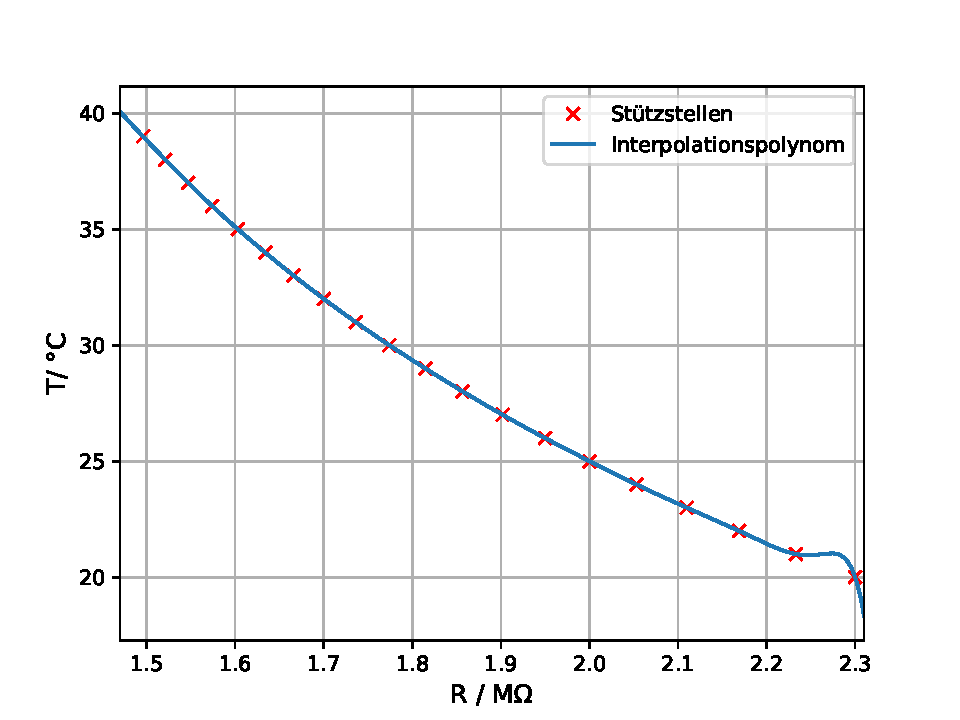
\includegraphics[width = 0.8\textwidth]{../Messdaten/temperature_fit.pdf}
  \caption{Graphische Darstellung der Polynominterpolation des Zusammenhangs zwischen Thermowiderstand $R$ und Temperatur $T$.}
  \label{fig: poly}
\end{figure}
 Die mit dem Interpolationspolynom berechneten
Temperaturen sind ebenfalls in Tabelle \ref{tab: data} eingefügt. Der Zusammenhang zwischen der Viskosität von Luft $\eta$ und
der Temperatur $T$ wird der Anleitung \cite{anleitung503} entsprechend als linear angenommen. Mit den Wertepaaren
\begin{align}
  \eta_1 &= \SI{1.85e-5}{\newton\second\meter^{-2}}, \quad T_1 = \SI{16}{\celsius} \\
  \eta_2 &= \SI{1.88e-5}{\newton\second\meter^{-2}}, \quad T_2 = \SI{32}{\celsius},
\end{align}
die dem Graphen aus der Anleitung entnommen werden, wird eine Geradengleichung bestimmt, die den Temperaturen
$T$ in $\si{\celsius}$ die Viskositäten $\eta$ in $\si{\newton\second\meter^{-2}}$ zuordnet.
\begin{equation}
  \eta(T) = \SI{0.0019}{\newton\second\meter^{-2} \celsius^{-1} } \cdot  T  + \SI{1.82}{\newton\second\meter^{-2}}.
\end{equation}
Die somit berechneten Viskositäten sind in Tabelle \ref{tab: data} aufgetragen.
Die Fallgeschwindigkeiten der Tröpfchen berechnen sich gemäß $v = s/t$ und der Falldistanz $s = \SI{0.5}{\milli\meter}$.
Mit den Gleichungen \eqref{eq:radius_teilchen} und \eqref{eq:q} ergeben sich somit schließlich die Tröpfchenradien $r$ und Ladungen $q$. Hierbei wird
direkt die Korrektur \eqref{eq:q_korri} angewandt. Für den Luftdruck wird konstant der Atmosphärendruck von
$\SI{1.0132}{\bar}$ angenommen. Alle Ergebnisse sind in Tabelle \ref{tab: data} eingetragen. \\
\begin{table} 
\centering 
\caption{Gemessene und brechnete Größen für einzelne beobachtete Tropfen. Thermowiderstand $R$, Temperatur $T$, Luftviskosität $\eta$, Tröpfchenradius $r$, Fallzeit $t$, Fallgeschwindigkeit $v_0$, Schwebespannung $U$ und korrigierte Ladung $q$.} 
\label{tab: data} 
\begin{tabular}{S S S S S S S S } 
\toprule  
{$R/\si{\mega\ohm}$} & {$T/\si{\celsius}$} & {$\eta/10^{-5}\si{\newton\second\meter^{-2}}$} & {$r/\si{\milli\meter}$} & {$t/\si{\second}$} &
 {$v_0/\si{\centi\meter\second^{-1}}$} & {$U/\si{\volt}$}  & {$q/10^{-19}\si{\coulomb}$}  \\ 
\midrule  
 1.89  & 27.26  & 0.00  & 0.00  & 10.525  & 0.005  & 79.60  & 9.19\\ 
1.88  & 27.48  & 0.00  & 0.00  & 11.498  & 0.004  & 68.80  & 9.25\\ 
1.85  & 28.17  & 0.00  & 0.00  & 10.807  & 0.005  & 61.50  & 11.43\\ 
1.83  & 28.63  & 0.00  & 0.00  & 9.504  & 0.005  & 144.00  & 5.98\\ 
1.81  & 29.11  & 0.00  & 0.00  & 9.251  & 0.005  & 143.60  & 6.26\\ 
1.81  & 29.11  & 0.00  & 0.00  & 12.489  & 0.004  & 97.90  & 5.72\\ 
1.81  & 29.11  & 0.00  & 0.00  & 5.147  & 0.010  & 86.60  & 26.02\\ 
1.80  & 29.36  & 0.00  & 0.00  & 28.793  & 0.002  & 22.30  & 6.57\\ 
1.79  & 29.60  & 0.00  & 0.00  & 16.228  & 0.003  & 130.40  & 2.83\\ 
1.79  & 29.60  & 0.00  & 0.00  & 15.588  & 0.003  & 70.20  & 5.61\\ 
1.78  & 29.85  & 0.00  & 0.00  & 4.940  & 0.010  & 184.40  & 13.04\\ 
1.77  & 30.11  & 0.00  & 0.00  & 23.773  & 0.002  & 26.70  & 7.50\\ 
1.77  & 30.11  & 0.00  & 0.00  & 16.099  & 0.003  & 280.00  & 1.34\\ 
1.76  & 30.36  & 0.00  & 0.00  & 10.014  & 0.005  & 98.60  & 8.07\\ 
1.76  & 30.36  & 0.00  & 0.00  & 21.332  & 0.002  & 207.00  & 1.15\\ 
1.76  & 30.36  & 0.00  & 0.00  & 10.561  & 0.005  & 79.70  & 9.18\\ 
1.75  & 30.62  & 0.00  & 0.00  & 13.247  & 0.004  & 53.80  & 9.50\\ 
1.75  & 30.62  & 0.00  & 0.00  & 13.929  & 0.004  & 104.40  & 4.52\\ 
1.74  & 30.89  & 0.00  & 0.00  & 7.828  & 0.006  & 197.00  & 5.95\\ 
1.74  & 30.89  & 0.00  & 0.00  & 13.804  & 0.004  & 301.00  & 1.59\\ 
1.74  & 30.89  & 0.00  & 0.00  & 15.460  & 0.003  & 35.00  & 11.42\\ 
1.74  & 30.89  & 0.00  & 0.00  & 9.605  & 0.005  & 83.40  & 10.19\\ 
1.73  & 31.16  & 0.00  & 0.00  & 16.007  & 0.003  & 60.60  & 6.24\\ 
1.73  & 31.16  & 0.00  & 0.00  & 14.304  & 0.003  & 97.10  & 4.66\\ 
1.73  & 31.16  & 0.00  & 0.00  & 13.946  & 0.004  & 107.90  & 4.37\\ 
\bottomrule 
\end{tabular} 
\end{table}

\subsection{Bestimmung der Elementarladung}
Um nun die Elementarladung aus den gewonnen Daten zu ermitteln wird wie folgt vorgegangen. Alle bestimmten
Ladungen sollten der Theorie zur Folge ein ganzzahliges Vielfaches von $\mathup{e}\ua{0}$ sein, das heißt für die %\map{e}
Tröpfenladungen $q\ua{i}$ muss gelten
\begin{equation}
  \mathup{rd}\ua{0}\left(\frac{q\ua{i}}{\mathup{e}\ua{0}}\right) - \frac{q\ua{i}}{\mathup{e}\ua{0}} = 0 \quad \forall\, \mathup{i}.
  \label{eq: rundung}
\end{equation}
Hierbei entspricht $\mathup{rd}\ua{0}$ der Rundung auf eine ganze Zahl. Für jede ermittelte Ladung wird nun diejenige
Ladung berechnet, die \eqref{eq: rundung} minimal werden lässt. Dazu werden aus einer diskreten Menge $q\ua{e}$ Werte entnommen
und jeweils in \eqref{eq: rundung} eingesetzt. Für jede Ladung $q\ua{i}$ ergibt sich somit eine Ladung $\mathup{e}\ua{i} \in q\ua{e}$ mit
\begin{equation}
  \left|\mathup{rd}\ua{0}\left(\frac{q\ua{i}}{\mathup{e}\ua{i}}\right) - \frac{q\ua{i}}{\mathup{e}\ua{i}}\right| \,\leq\,
  \left|\mathup{rd}\ua{0}\left(\frac{q\ua{i}}{q}\right) - \frac{q\ua{i}}{q} \right| \quad \forall q \in q\ua{e}.
\end{equation}
Der Mittwert über alle so bestimmten Ladungen liefert eine Näherung für die Elementarladung.\\
Zunächst muss eine grobe Abschätzung für das Intervall $q\ua{e}$ gefunden werden. Hierzu wird ausgenutzt, dass die Elementarladung
kleiner oder gleich der kleinsten Differenz zwischen zwei ungleichen Ladungen aus der Messreihe sein muss. Um auszuschließen, dass
der Datensatz der bestimmten Tröpfchenladungen Zahlenwerte enthält, die aufgrund von Messungenauigkeiten unterhalb
der unbekannten Elementarladung liegen, werden die kleinsten $\SI{20}{\percent}$ (hier also die 5 kleinsten Ladungen in \ref{tab: data}, rot dargestellt)
aus der Betrachtung ausgeschlossen. Es wird mit den verbliebenen Ladungen das Minimum der Menge
\begin{equation}
  d\ua{q} = \left\{ \left| q\ua{i} - q\ua{j}\right| \quad \forall  \mathup{i}, \mathup{j} \, \quad \mathup{i} \neq \mathup{j}   \right\}
\end{equation}
bestimmt. Um auszuschließen, dass diese diskrete Menge auch solche Ladungsdifferenzen enthält, die im Rahmen der Messungenauigkeit
kleiner als die Elementarladung sind (etwa weil zwei Tröpchen die selbe Ladung tragen), werden auch hier die kleinsten $\SI{20}{\percent}$ der möglichen Differenzen ausgeschlossen.
Es berechnet sich oberhalb dieser Schranke die kleinste Differenz zu
\begin{equation}
  d\ua{min} = \SI{1.67e-19}{\coulomb}.
\end{equation}
Als diskrete Menge $q\ua{e}$ wird nun folgendes feines Raster angesetzt
\begin{equation}
  q\ua{e} = \left\{ d\ua{min} - \SI{e-19}{\coulomb}  +  \frac{2\mathup{i} \cdot \SI{e-19}{\coulomb}}{\mathup{m}}, \quad \mathup{i} = 0, \dots, \mathup{m}     \right\}\quad \text{mit} \, \,\mathup{m} = 1000.
\end{equation}
Das Intervall erstreckt sich also in einem Abstand von $\SI{e-19}{\coulomb}$ um die kleinste Ladungsdifferenz und sollte deshalb die Elementarladung enthalten.
Nun werden alle Ladungen des Intervalls für jede Ladung $q\ua{i}$ in Gleichung \eqref{eq: rundung} eingesetzt und jeweils die jenige Ladung bestimmt,
die die Rundungsdifferenz minimal werden lässt. Die Ergebnisse sind in Tabelle \ref{tab: q_best} eingetragen. Abbildung \ref{fig: streuung} zeigt die Streuung
der so ermittelten Ladungen um die Elementarladung. Als Mittelwert mit zugehöriger Standardabweichung ergibt sich
\begin{equation}
  \mathup{e}\ua{exp} = \SI{+1.8(1)e-19}{\coulomb}.
\end{equation}
Dieses Ergebnis weicht vom Literaturwert
\begin{equation}
  \mathup{e}\ua{0} = \SI{1.6021766208e-19}{\coulomb}
\end{equation}
im Mittel um $\SI{11}{\percent}$ ab. Zum Abschluss der Auswertung sei angemerkt, dass eine volle Betrachtung des Datensatzes ohne
die gewählten Aussparungen folgenden Wert für die Elementarladung liefert
\begin{equation}
   \mathup{e}'\ua{exp} = \SI{+0.8(11)e-19}{\coulomb}.
\end{equation}
\begin{table}[H] 
\centering 
\caption{Verwendete Tröpfchenladungen $q_{i}$ zur Bestimmung der Elementarladung und jeweils berechnete Minimalstelle $e_{i}$ der Gleichung \eqref{eq: rundung}.} 
\label{tab: q_best} 
\begin{tabular}{S S } 
\toprule  
{$q_{i} /\SI{e-19}{\coulomb}$} & {$e_{i} /\SI{e-19}{\coulomb}$}  \\ 
\midrule  
 4.52  & 2.26\\ 
4.66  & 2.33\\ 
5.61  & 1.87\\ 
5.72  & 1.91\\ 
5.95  & 1.49\\ 
5.98  & 1.20\\ 
6.24  & 1.56\\ 
6.26  & 1.04\\ 
6.57  & 2.19\\ 
7.50  & 2.50\\ 
8.07  & 1.34\\ 
9.18  & 0.71\\ 
9.19  & 2.30\\ 
9.25  & 1.16\\ 
9.50  & 1.58\\ 
10.19  & 1.70\\ 
11.42  & 0.67\\ 
11.43  & 2.29\\ 
13.04  & 1.86\\ 
26.02  & 1.53\\ 
\bottomrule 
\end{tabular} 
\end{table}
\begin{figure}[H]
  \centering
  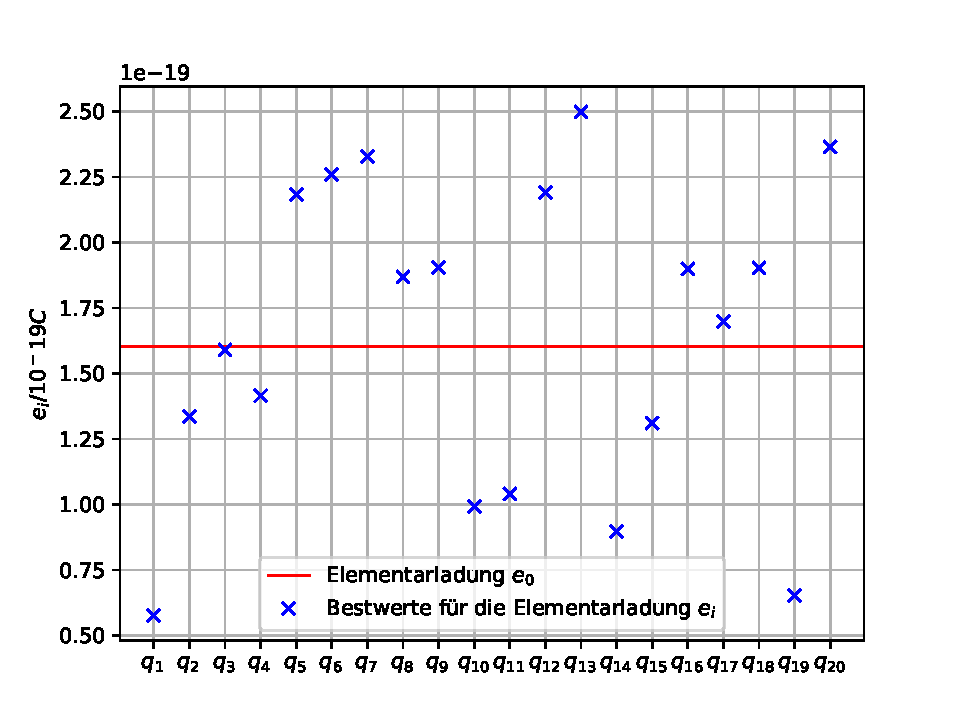
\includegraphics[width = 0.8\textwidth]{../Messdaten/scattering.pdf}
  \caption{Graphische Darstellung der Streung der ermittelten Bestwerte $\mathup{e}\ua{i}$ zu jeder Ladung $q\ua{i}$ um die Elementarladung $\mathup{e}_0$.}
  \label{fig: streuung}
\end{figure}
